\section{Window Layout Concept}
    Developers can define their working environment to fit the needs and preferences. For a better understanding of further comments and instructions, five major screen areas are defined. % popsáno v obrázku


   \begin{figure}[h]
        \centering
        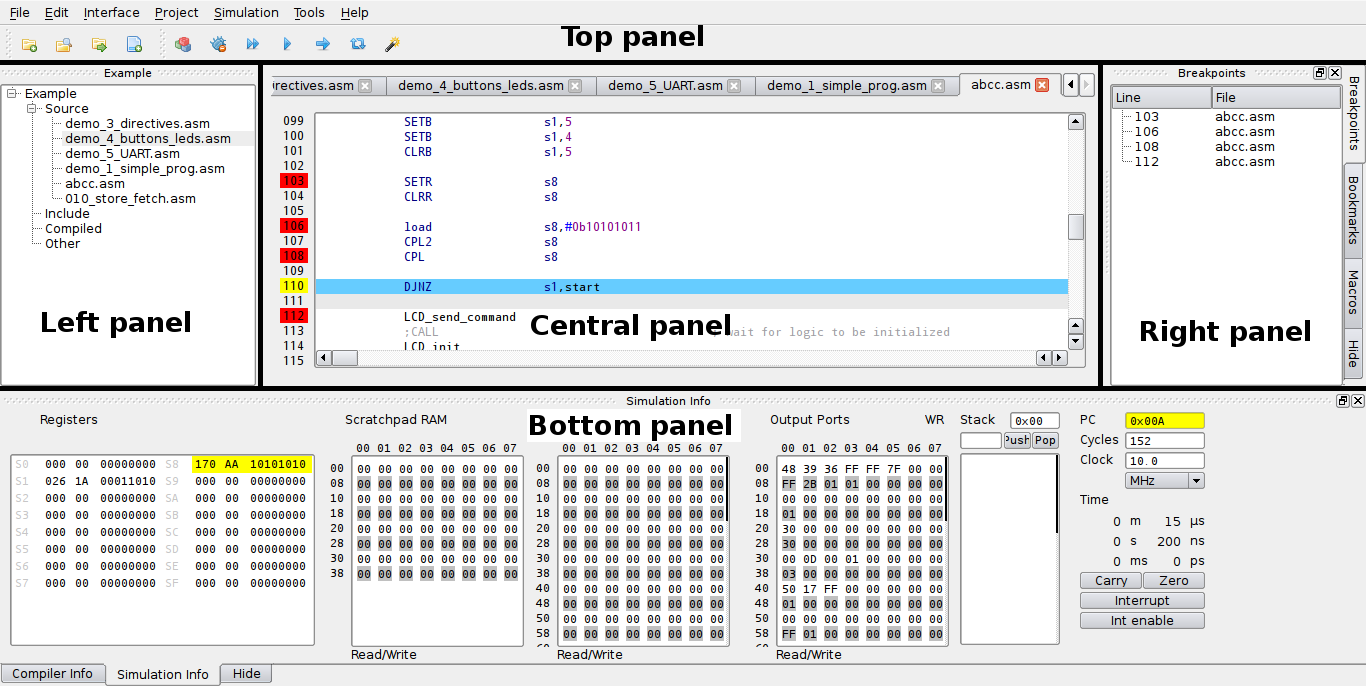
\includegraphics[width=\textwidth]{img/Main_window.png}
        \caption{Window layout concept}
    \end{figure}

\subsection{Middle panel}
    Middle panel is main text editor for writing a code. It has syntax highligh for better readability and you can easily
    add breakpoints and bookmarks just by clicking on desired line number.

\subsection{Top panel}

   \begin{figure}[h!]
        \centering
        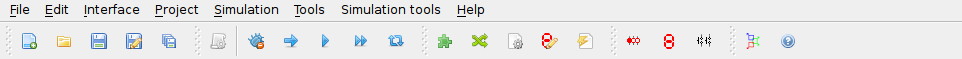
\includegraphics[width=0.75\textwidth]{img/top_panel.png}
        \caption{Top panel icons}
    \end{figure}

    \subsubsection{Top panel icons}
        \begin{itemize}
            \item New project: Creates a new project.
            \item Open project: Allows to open an existing project file.
            \item Save project: Saves current project file.
            \item Compile: Compiles your code.
            \item Start Simulation: Enters simulation mode.
            \item Run: Simulation at full speed.
            \item Animate: Simulation with updated GUI.
            \item Step: Performs one step.
            \item Reset: Resets simulation to its initial state.
            \item Unhighlight: You can erase highlighted text.
        \end{itemize}

        
    \begin{table}[h!]
        \begin{tabular}{cc}
            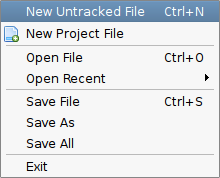
\includegraphics[width=.25\textwidth]{img/NewImg/file.png}
                &
            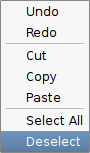
\includegraphics[width=.25\textwidth]{img/NewImg/edit.png}
                \\
            File & Edit
        \end{tabular}
    \end{table}

    \begin{table}[h!]
        \begin{tabular}{cc}
            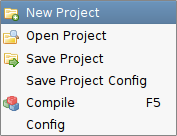
\includegraphics[width=.25\textwidth]{img/NewImg/project_tab.png}
                &
            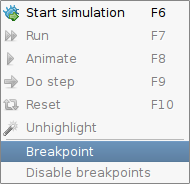
\includegraphics[width=.25\textwidth]{img/NewImg/simulation.png}
                \\
            Project & Simulation
        \end{tabular}
    \end{table}
 
    \subsubsection{Top panel}
        \begin{itemize}
            \item Undo: will undo all edit actions on the open document in reverse order
            \item Redo: will redo all undo actions
            \item Cut: cuts all selected parts of the open doecument and puts it on the clipboard
            \item Copy: copies all selected parts of the open document to the clipboard
            \item Paste: pastes the text contents of the clipboard in the open document
            \item Select: All selects all text in the open document
            \item Find: find a to be given string through the open document
            \item Replace: replace a given string in the open document by a new string
        \end{itemize}
    
    \subsubsection{Top panel}
        \begin{itemize}
            \item Undo: will undo all edit actions on the open document in reverse order
            \item Redo: will redo all undo actions
            \item Cut: cuts all selected parts of the open doecument and puts it on the clipboard
            \item Copy: copies all selected parts of the open document to the clipboard
            \item Paste: pastes the text contents of the clipboard in the open document
            \item Select: All selects all text in the open document
            \item Find: find a to be given string through the open document
            \item Replace: replace a given string in the open document by a new string
        \end{itemize}

    \subsubsection{Top panel}
        \begin{itemize}
            \item Undo: will undo all edit actions on the open document in reverse order
            \item Redo: will redo all undo actions
            \item Cut: cuts all selected parts of the open doecument and puts it on the clipboard
            \item Copy: copies all selected parts of the open document to the clipboard
            \item Paste: pastes the text contents of the clipboard in the open document
            \item Select: All selects all text in the open document
            \item Find: find a to be given string through the open document
            \item Replace: replace a given string in the open document by a new string
        \end{itemize}



\subsection{Bottom panel}
    Here you can see bottom panel. You can see status of internal registers, scratchpad ram, input and output ports, stack, program counter, elapsed time and cycles, actual clock and internal flags: CARRY and ZERO. All those features can be edited during processor simulation. 

   \begin{figure}[h!]
        \centering
        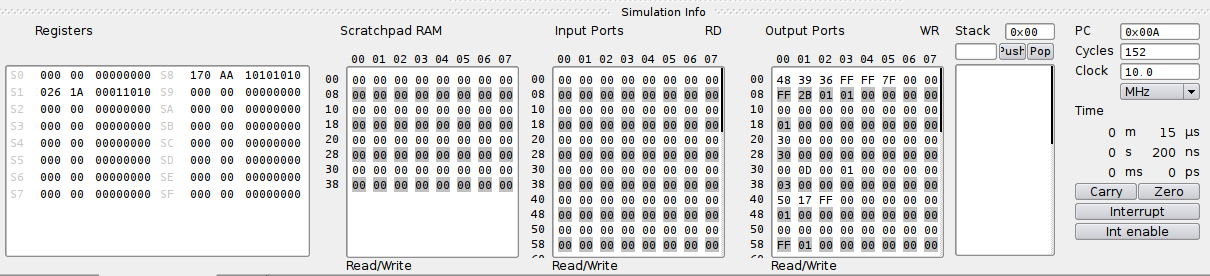
\includegraphics[width=\textwidth]{img/bottom_panel.png}
        \caption{Window layout concept}
    \end{figure}

\subsection{Right panel}
    Right panel contains list of breakpoints and bookmarks. Yoou can also find here list of symbols and macros in your source code.
    
\subsection{Left panel}
    Here you can see main project tree. You can close or configure project. Also add file or create a new one. You can also see included file or open
    compiled files like .LST for better debuging.

    \begin{table}[h!]
        \begin{tabular}{cc}
            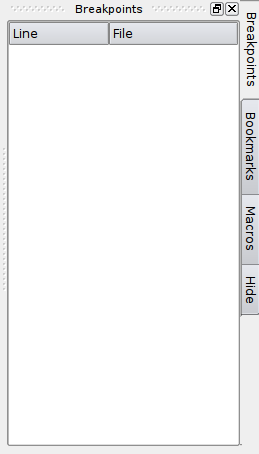
\includegraphics[width=.33\textwidth]{img/right_panel.png}
                &
            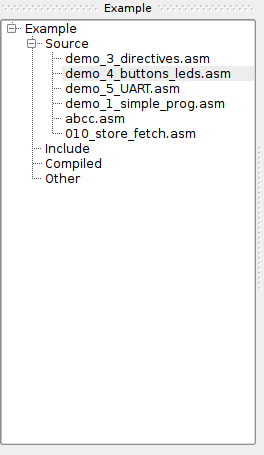
\includegraphics[width=.33\textwidth]{img/left_panel.png}
                \\ 
            Right panel & Left panel
        \end{tabular}
    \end{table}

    
\clearpage
\enlargethispage{6\baselineskip}
\subsection{Project configuration}
    In project configuration window, you can edit project and compiler settings. You can open project configuration window by right clicking to project name in the left panel. See the pictures below.
    This will open main configuration window with multiple tabs on the left side.

    \subsubsection{Project - Options}
        \begin{itemize}
            \item Project name: Name of your project.
            \item Architecture: Select which architecture is project using.
            \item Family: Select processor family of selected architecture.
            \item Infopanel: Brief description of selected processor.
        \end{itemize}
    
        \subsubsection{Project - Memory}
            \begin{itemize}
                \item Size options: Tell compiler limits of your processor data and program memory.
                \item Interrupt vector: You can change interrupt vector ( program memory - 1 is max),
                \item HW build: Number of your HW build.
            \end{itemize}
    
        \begin{table}[h!]
            \begin{tabular}{cc}
                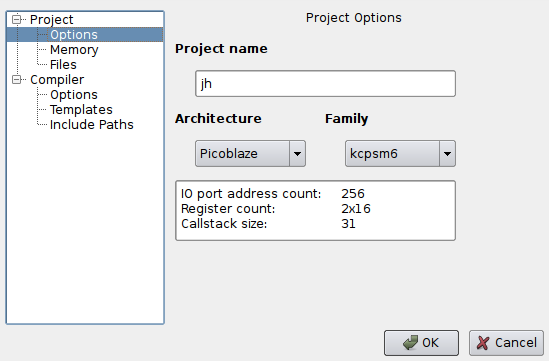
\includegraphics[width=.5\textwidth]{img/NewImg/config2.png}
                    &
                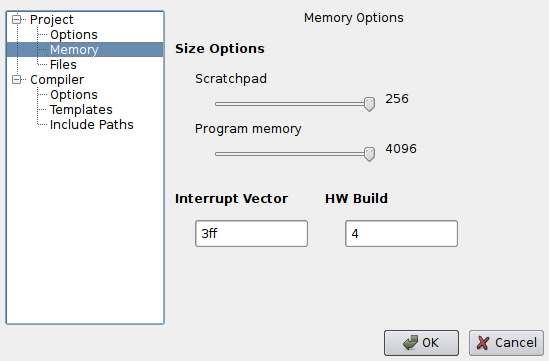
\includegraphics[width=.5\textwidth]{img/NewImg/config1.png}
                    \\
                Project - Options & Project - Memory
            \end{tabular}
        \end{table}

        \clearpage
        \subsubsection{Project - Files}
        Here is where you can create, add or delete project files. You can also set your main file.

        \subsubsection{Compiler - Options}
            \begin{itemize}
                \item Main file: If you have "Use main file" checked, you can choose which file will be main.
                \item Generate: Selection of files created after compilation.( in your project folder )
            \end{itemize}

        \begin{table}[h!]
            \begin{tabular}{cc}
                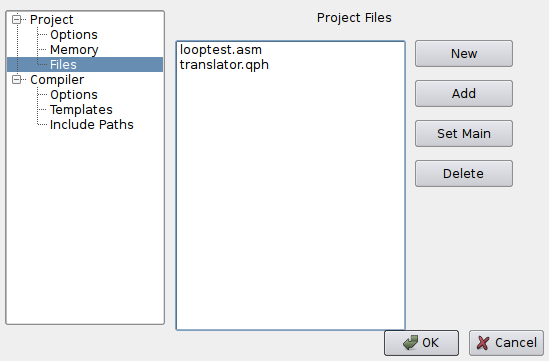
\includegraphics[width=.5\textwidth]{img/NewImg/config3.png}
                    &
                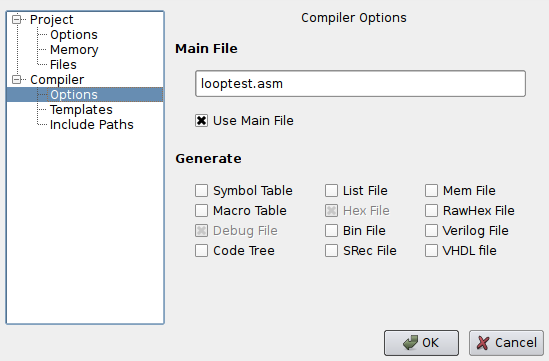
\includegraphics[width=.5\textwidth]{img/NewImg/config4.png}
                    \\
                Project - Files & Compiler - Options
            \end{tabular}
        \end{table}

        \subsubsection{Compiler - templates}
        Here you can choose which template will be used. By default, MDS templates are being used.

        \subsubsection{Compiler - include paths}
            Here you can add or edit path, where will be compiler trying to find included files with directive INCLUDE. 

        \begin{table}[h!]       
            \begin{tabular}{cc}
                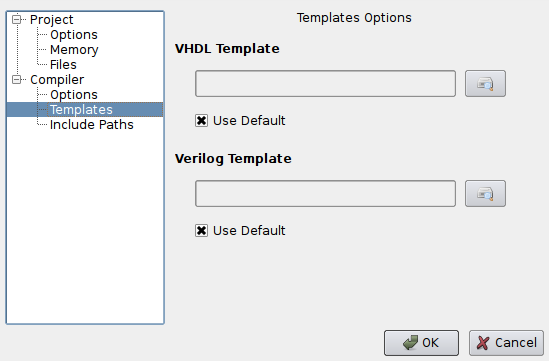
\includegraphics[width=.5\textwidth]{img/NewImg/config5.png}
                    &
                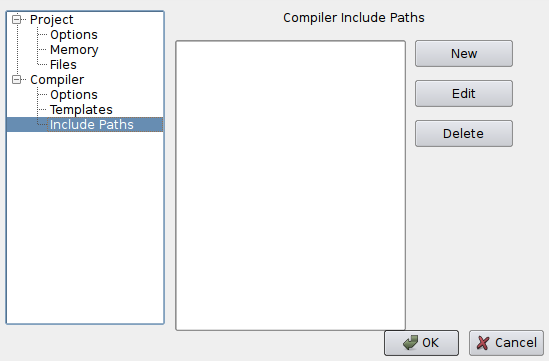
\includegraphics[width=.5\textwidth]{img/NewImg/config6.png}
                    \\
                Compiler - Templates & Compiler - Include paths
            \end{tabular}
            \end{table}

\subsection{Interface configuration}
    In interface configuration window, you can edit IDE behavior and appearance, editor settings like fonts, tab width and encoding or simulator warnings.
    You can open interface configuration clicking on top panel ( interface -> config ).This will open interface configuration window with
    multiple tabs on the left side. See the pictures below.

    \subsubsection{IDE - General}
        Main settings of IDE. You can set if you want splash screen, tips on start-up, session restoration or change language of whole IDE.

    \subsubsection{Editor - General}
        General settings of IDE editor. You can set tab width, number of spaces .

        \begin{table}[h!]
            \begin{tabular}{cc}
                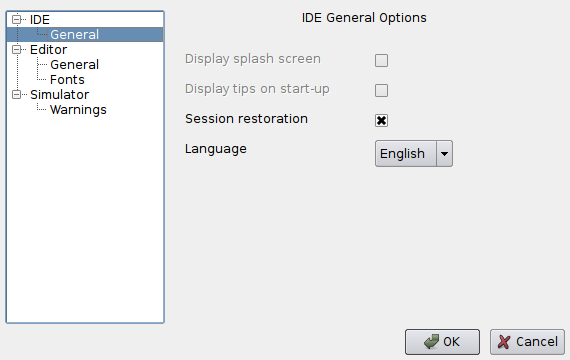
\includegraphics[width=.5\textwidth]{img/NewImg/interface1.png}
                    &
                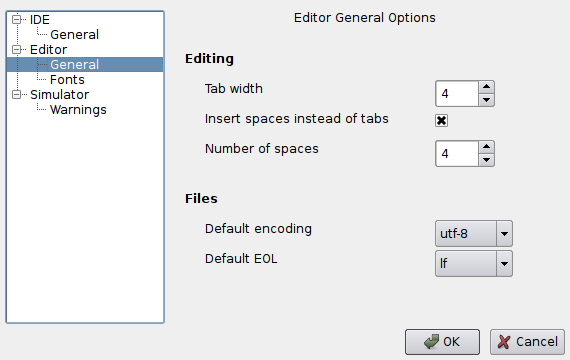
\includegraphics[width=.5\textwidth]{img/NewImg/interface2.png}
                    \\
                IDE - General & Editor - General
            \end{tabular}
        \end{table}

        \begin{table}[h!]
            \begin{tabular}{cc}
                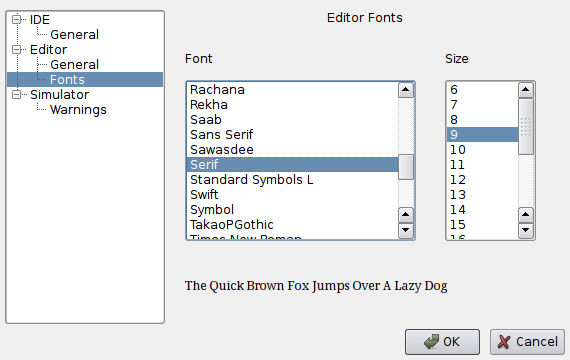
\includegraphics[width=.5\textwidth]{img/NewImg/interface3.png}
                    &
                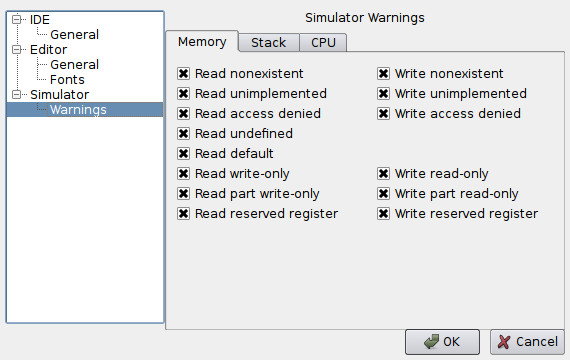
\includegraphics[width=.5\textwidth]{img/NewImg/interface4.png}
                    \\
                Editor - Fonts & Simulator - Warnings -> Memory
            \end{tabular}
        \end{table}

        \begin{table}[h!]
            \begin{tabular}{cc}
                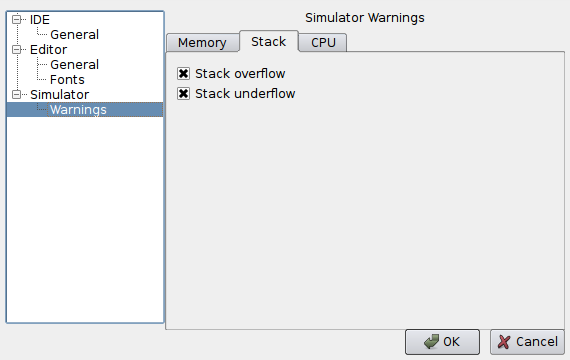
\includegraphics[width=.5\textwidth]{img/NewImg/interface5.png}
                    &
                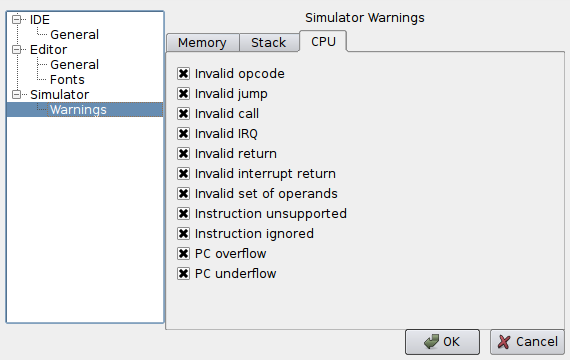
\includegraphics[width=.5\textwidth]{img/NewImg/interface6.png}
                    \\
                Simulator - Warnings -> Stack & Simulator - Warnings -> CPU
            \end{tabular}
        \end{table}

        
\subsection{Other tools}

\subsection{DATA file convertor}
    This tool alows you to convert selected data file to another. Mutual conversion can be made with Hex, Bin, SRec, XilMem, XilVerilog and XilVhdl.
    \begin{description}
        \item[Section Input File] Here you can select desired input data file which is going to be converted
        \item[Section Input Options] In this section, you define what type of input file is going to be converted
        \item[Input file type] Available options - Hex, Bin, SRec, XilMem, XilVerilog and XilVhdl
        \item[Bytes per record] Only if you want to convert XilMem file. Defines number of bytes per record
        \item[OPCode size] Defines opcode size of selected data file. Available are 16 and 18
        \item[Section Output File] Defines target
        \item[Section Output Options] Here you can select desired output data file.
        \item[Input file type] Available options - Hex, Bin, SRec, XilMem, XilVerilog and XilVhdl.
        \item[Tab size]  Define number of inserted spaces when you press Tab.
        \item[Short instructions] Here you can allow short instructions like LD, RETI or others
    \end{description}

    \begin{figure}[h]
        \centering{}
        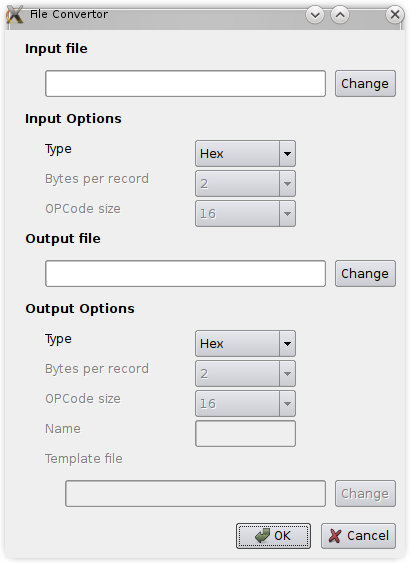
\includegraphics[width=.5\textwidth]{img/DATA_convertor.png}
        \caption{DATA file convertor}
    \end{figure}

\subsection{ASM translator}
    With this tool, you can translate your previously written assembler code in different syntax.
    You can sellect one of three choices - Xilinx, Mediatronix and OpenPicIde. Input code should be without
    errors.
    \begin{description}
        \item[Section Input File] Here you can choose which file you want to translate into the MDS assembler
        \item[Section ASM type] Input file syntax version. Translator needs to know input file syntax. Select one of three choices - Xilinx, Mediatronix and OpenPicIde
        \item[Symbol] Case of symbols - UPPERCASE or LOWERCASE
        \item[End of line] Indentation - Choose between Tabs or Spaces
        \item[Directive] Case of Directives - UPPERCASE or LOWERCASE
        \item[Indentation] Three choices - Tabs, Spaces and Keep (indentation unchanged)
        \item[Instruction] Case of instructions - UPPERCASE or LOWERCASE
        \item[Tab size]  Define number of inserted spaces when you press Tab.
        \item[Short instructions] Here you can allow short instructions like LD, RETI or others
    \end{description}

    \begin{figure}[h]
        \centering{}
        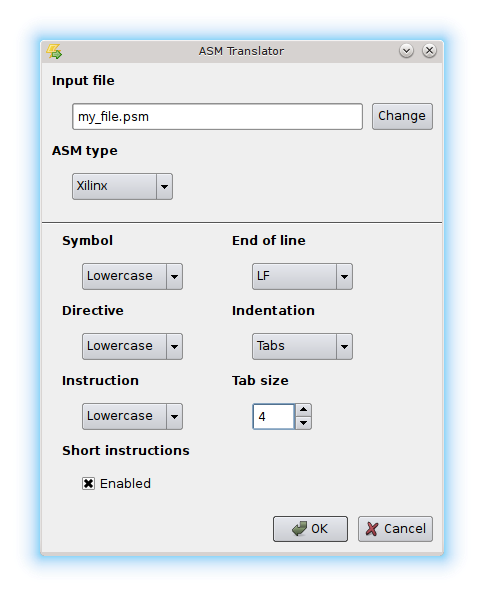
\includegraphics[width=.5\textwidth]{img/ASM_translator.png}
        \caption{ASM translator}
    \end{figure}

\subsection{Disassembler}
    A disassembler is a tool that translates machine language into assembly language. The inverse
    operation to that of an assembler.

    \begin{description}
        \item[Section File] Here you can choose which file you want to be disassembled
        \item[Section Target] Architecture - Select processor architecture
        \item[Family] select processor family of selected architecture
        \item[Section Options] Indentation - Choose between Tabs or Spaces
        \item[TabSize] Number of spaces in one tab
        \item[Radix] Binary,Octal, Decima or Hexadecimal
        \item[Linebreak] LF,CR or CRLF
        \item[Case]  You can choose if you want disassemled file will be in upper or lower case
        \item[Generate symbols] Select which symbols should be disassembled
    \end{description}

    \begin{figure}[h]
        \centering{}
        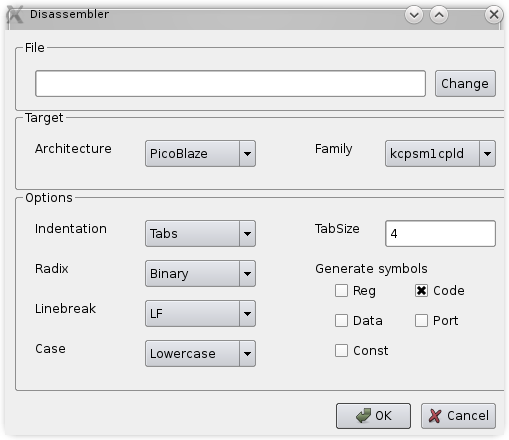
\includegraphics[width=.5\textwidth]{img/disassembler_window.png}
        \caption{Disassembler}
    \end{figure}

\subsection{Waiting loop generator}
    In many cases, it is usefull to have a tool for creating waiting loops. It can save some time in development process. This tool can generate
    waiting loops using up to six registers. All you have to do is insert desired waiting time or number of cycles and valid frekvency.

    \begin{description}
        \item[Section Input variable] You can choose between time or cycles
        \item[Section Desired waiting time] Insert number of executed time or cycles 
        \item[Section Frekvency] Set working frekvency 
        \item[Section Register names] Optional selection. You can change register names in generated code
        \item[Section Generated code] Here is where code will appear
        \item[Instruction] Select instruction used in loop.
        \item[Type] Type of waiting loop you want to create (blank/macro).
        \item[Checkboxes UpperCase and Comments]  You can turn off automaticaly added comments or change letter case
        \item[Button Copy to clipboard] This will copy loop into your clipboard
        \item[Button Generate] When you have all set. This will generate loop
    \end{description}

    \begin{figure}[h]
        \centering{}
        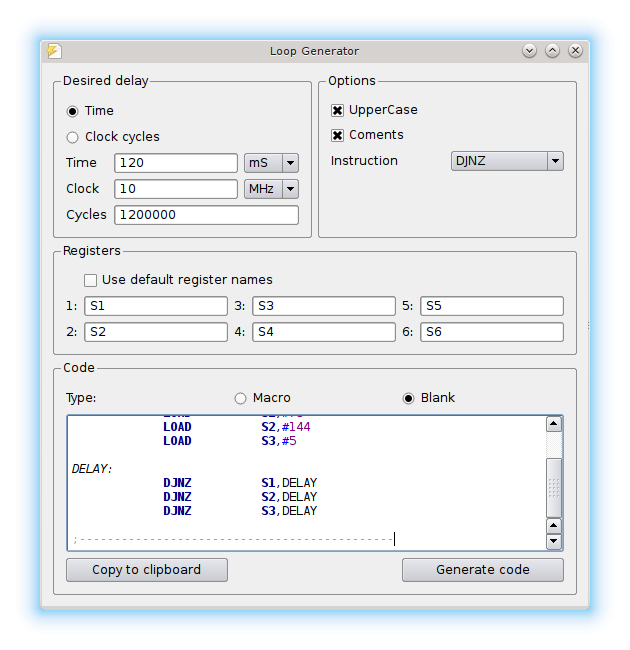
\includegraphics[width=.7\textwidth]{img/loop_gen.png}
        \caption{Loop generator user interface}
    \end{figure}

\subsection{8-segment editor}
    \begin{wrapfigure}{r}{0pt}
        \centering{}
        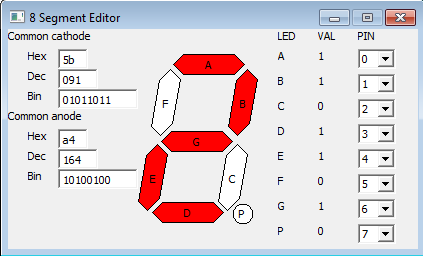
\includegraphics[width=110pt]{img/8segment.png}
        \caption{8-segment editor}
    \end{wrapfigure}
    With this tool you can easily determine what value you have to set on a port to display a digit on a numerical LED display. In the left part of the dialog window, you can find numerical val ues corresponding to the digit displayed in the middle part. These values are represented for both common cathode and anode and in three numerical bases, hexadecimal, decimal and oc tal. Buttons on left side from entry boxes copies value from adjacent entry box into clipboard. In the right part of the window you can set what port pin is connected to what LED segment.

\subsection{Number base converter}
    \begin{wrapfigure}{r}{0pt}
            \centering
            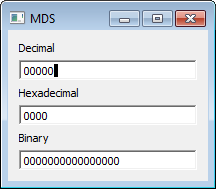
\includegraphics[width=90pt]{img/convertor.png}
            \caption{Convertor}
    \end{wrapfigure}
    This tool is very usefull, when you want to find out the representation of given number in other number bases.










    